\section{Intervals}

In mathematics, intervals are a fundamental concept used to represent sets of real numbers. They are commonly used to describe domains of functions, solutions to inequalities, and other mathematical concepts. Intervals come in several forms, each with its own notation and meaning.

\subsection{Open Interval: (a, b)}

An open interval between two numbers, $a$ and $b$, is represented as $(a, b)$. It includes all real numbers greater than $a$ and less than $b$, excluding the endpoints $a$ and $b$ themselves. In mathematical notation, this can be expressed as:

$$(a, b) = \{x \in \mathbb{R} \mid a < x < b\}$$

For example, $(1, 3)$ represents all real numbers greater than 1 and less than 3, but it does not include 1 and 3.
It is also really important to note that the smallest value MUST go on the left, and the largest value MUST go on the right. For example, $(3, 1)$ is not a valid interval because 3 is bigger than 1.

\subsection{Closed Interval: [a, b]}

A closed interval between two numbers, $a$ and $b$, is represented as $[a, b]$. It includes all real numbers greater than or equal to $a$ and less than or equal to $b$, including the endpoints $a$ and $b$. In mathematical notation, this can be expressed as:

$$[a, b] = \{x \in \mathbb{R} \mid a \leq x \leq b\}$$

For example, $[1, 3]$ represents all real numbers greater than or equal to 1 and less than or equal to 3, including 1 and 3.

\subsection{Half-Open or Half-Closed Intervals: [a, b) and (a, b]}

Half-open or half-closed intervals are intervals that include one endpoint but not the other. They are represented as $[a, b)$ and $(a, b]$.

- $[a, b)$ includes all real numbers greater than or equal to $a$ and less than $b$, including $a$ but not $b$.
- $(a, b]$ includes all real numbers greater than $a$ and less than or equal to $b$, including $b$ but not $a$.

For example, $[1, 3)$ represents all real numbers greater than or equal to 1 and less than 3, including 1 but not 3. $(1, 3]$ represents all real numbers greater than 1 and less than or equal to 3, including 3 but not 1.

\subsection{Infinite Intervals: $(-\infty, a)$ and $(a, \infty)$}

Infinite intervals are used to represent unbounded sets of real numbers. They are represented as $(-\infty, a)$ and $(a, \infty)$.

- $(-\infty, a)$ includes all real numbers less than $a$.
- $(a, \infty)$ includes all real numbers greater than $a$.

For example, $(-\infty, 1)$ represents all real numbers less than 1 (negative infinity to 1), and $(1, \infty)$ represents all real numbers greater than 1 (1 to positive infinity).

\subsection{Combining Intervals: Union ($\cup$)}

You can combine multiple intervals using the union symbol ($\cup$) to represent a domain that includes multiple disjoint intervals. For example, if you have the intervals $(1, 3)$ and $(5, 7)$, their union is represented as $(1, 3) \cup (5, 7)$, which includes all real numbers between 1 and 3 (excluding 1 and 3) and all real numbers between 5 and 7 (excluding 5 and 7).

In summary, intervals are a powerful tool in mathematics for representing sets of real numbers. Understanding the different types of intervals and their notations is essential for working with functions, inequalities, and various mathematical concepts.

\subsection{Examples}
\textbf{Example 1:} Translate these phrases into mathematical notations.
\begin{enumerate}
    \item All real numbers between 1 and 3, but not including 1 and 3.
          We can translate this in a couple of ways:
          \begin{itemize}
              \item $(1, 3)$
              \item $\{x \in \mathbb{R} \mid 1 < x < 3\}$
              \item Also with a number line. \\
                    \begin{tikzpicture}
                        % Draw the number line
                        \draw[<->] (0,0) -- (4,0); % Adjust the range as needed

                        % Mark 1 with an open circle
                        \draw[fill=white] (1,0) circle (2pt) node[below] {$1$};

                        % Mark 3 with an open circle
                        \draw[fill=white] (3,0) circle (2pt) node[below] {$3$};

                        % Interval notation
                    \end{tikzpicture}
          \end{itemize}
          When we using drilled circle we are stating that the number is not included in the interval. If it was included then we would use a solid(filled) circle.

    \item All real numbers greater than or equal to 1 and less than or equal to 3, including 1 and 3.
          We can translate this in a couple of ways:
          \begin{itemize}
              \item $[1, 3]$
              \item $\{x \in \mathbb{R} \mid 1 \leq x \leq 3\}$
              \item Also with a number line. \\
                    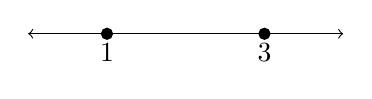
\begin{tikzpicture}
                        % Draw the number line
                        \draw[<->] (0,0) -- (4,0); % Adjust the range as needed

                        % Mark 1 with an open circle
                        \draw[fill=black] (1,0) circle (2pt) node[below] {$1$};

                        % Mark 3 with an open circle
                        \draw[fill=black] (3,0) circle (2pt) node[below] {$3$};

                        % Interval notation
                    \end{tikzpicture}
          \end{itemize}
          When we using filled circle we are stating that the number is included in the interval. If it was not included then we would use a drilled circle.
\end{enumerate}
Let's see a couple of examples for writing inequalities in interval notation and vice versa.

\begin{itemize}
    \item  $x \in (-\infty, 3)$
          \begin{itemize}
              \item This means that $x$ is any real number less than 3.
              \item We can also write this as $x < 3$.
          \end{itemize}
    \item $x \in [1, \infty)$
            \begin{itemize}
                \item This means that $x$ is any real number greater than or equal to 1.
                \item We can also write this as $x \geq 1$.
            \end{itemize}
    \item $4 \leq x \le 0$
            \begin{itemize}
                \item This means that $x$ is any real number between 4 and 0, including 4 and 0.
                \item We would write this as $x \in [4, 0]$. However this is not correct because the smallest value must go on the left and the largest value must go on the right. So we would write this as $x \in [0, 4]$.
            \end{itemize}
\end{itemize}

Notice that when dealing with infinity, the reason why we are using paranthesis is because infinity is not a number. It is a concept. So we can't include it in our interval. We can only approach it.
